% Alex Pinch, wasp poster for pollinator week mostly for myself
% June 21 2024

\documentclass[14pt]{extarticle}

\usepackage[T1]{fontenc}
\usepackage{graphicx}
\usepackage[export]{adjustbox}
\usepackage{tgbonum}
\usepackage{multicol}
\usepackage[dvipsnames]{xcolor}
    \definecolor{colour1}{HTML}{00F9DE}
\usepackage{geometry}
    \geometry{tmargin=1em,bmargin=2em,
lmargin=2em,rmargin=2em}

\begin{document}
\pagecolor{black}
\color{white}

%center title
\begin{center}\huge{**** PAUSE YOUR WASP HATE ****}\end{center}

\begin{multicols}{2}
\textcolor{black}{.} \\ % haha no idea how to put line breaks without some text before it
\noindent Wasps \textcolor{red}{aren't evil}. Many are territorial and their queens, commonly about in spring and fall, are protective of their eggs. \\\\
\noindent Wasps are \textcolor{colour1}{essential} to a healthy ecosystem. They prey on smaller insects and \textcolor{colour1}{pollinate}. Wasps enjoy their personal space: perhaps you were stung when close to a groundnest! 
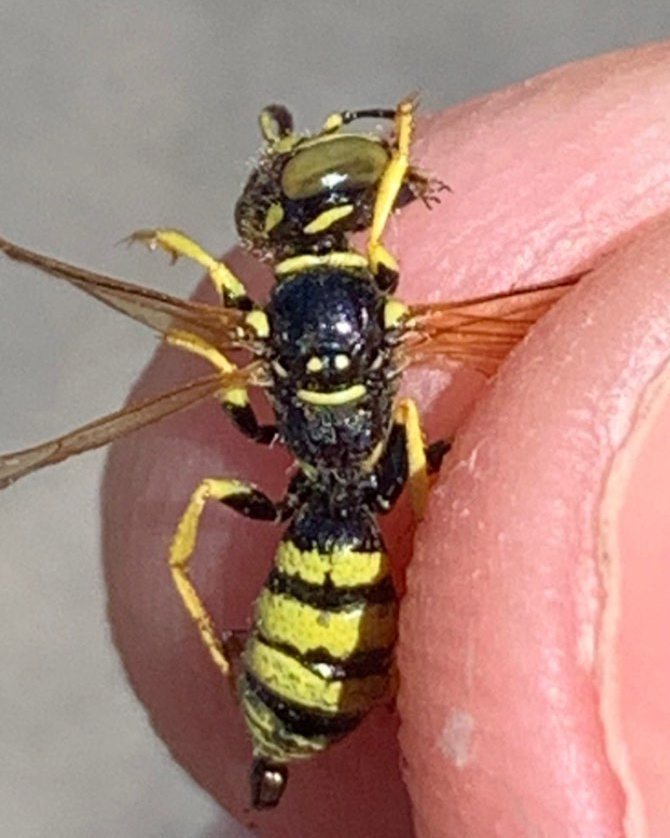
\includegraphics[width=0.35\textwidth, right]{wasp_smile.png}
\end{multicols}

%center phylogeny
\begin{center}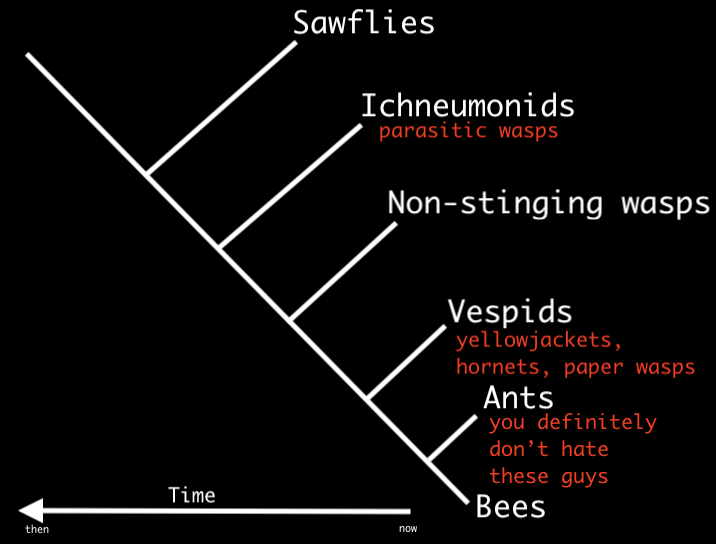
\includegraphics[width=0.65\textwidth,]{wasp_phylo.png}\end{center}

\noindent Ants and bees are close relatives of wasps. Bees ancestors were predatory, but wasps retained (and are excellent at) hunting. Some wasps can latch onto and \textcolor{colour1}{decapitate} their prey mid-air. \\\\
\noindent Wasp \textcolor{colour1}{diversity} is staggering. There are more species of ichneumonid wasps than \textcolor{colour1}{vertebrates} (that's every mammal, fish, bird, and reptile).\\\\
You may resume hating when the next vespid stings you unprovoked— that may be longer than you think!

\end{document}